\section{Bridging Looplets and Finch: The Tensor Interface}

%
The Finch language provides descriptions of computations that iterate over a subset of a regular grid that is lexicographically ordered.
%
At this point, the reader might believe that compilation of a Finch program simply involves simply replacing for loops over a range with for loops over iterators, but Finch programs and data structures are sufficiently flexible that this impossible.
%
First, the Finch language interacts with multi-dimensional tensors whereas the Looplet abstraction is best suited towards iterators over a single dimension.
%
We require a bridge between the single dimensional iterators created from looplets and the mutli-dimensional abstractions common to tensor compilers.
%
Second, since the iteration order of a Finch program might not match that of a data structure (a discordant traversal), different iterators need to be requested for the same data depending on the traversal order of the program.
%
So we require a bridge that can provide different iteration orders depending on the context.
%
Third, since Finch programs can read and write to the same data, multi-dimensional tensors need to provide iterators for reading and writing as well as machinery to manage transition between these states.


To build our bridge, we embrace a set of abstractions: level formats/Fiber Trees, iteration context dependent instantiation of iterators, and tensor life cycles.
%
Our first abstraction mostly already exists in the literature: a manner of specifying a data structure for a multi-dimensional tensor out of data structures for single dimensional tensors~\cite{sze2017efficient,chou2022compilation, chou2018format}.
%
We recapitulate the essential details here.
%
Our next two abstractions add to to the first by providing a mechanism to use data structures generated by the first abstraction in a greater variety of contexts while maintaining per-dimension encapsulation of array data structures.
%
We introduce an interface to instatiate iterators in a variety of contexts in our programs and we introduce the lifecycle interface to manage when we read and write to multi-dimensional iterators.
%
These interfaces add to the level abstraction, expanding the types of data that they can express via mapping to looplets and expanding the contexts in which they can be used.
%
Previous efforts to compile a greater variety of sparse array programs left these bridges untouched ~\cite{henry_compilation_2021, won2023unified, senanayake2020sparse}.

\subsection{Level Abstraction}
Fiber-tree style tensor abstractions have been the subject of extensive study
\cite{sze2017efficient, chou2022compilation, chou2018format}.  The underlying
idea is to represent a multi-dimensional tensor as a nested vector
datastructure, where each level of the nesting corresponds to a dimension of the
tensor. Thus, a matrix would be represented as a vector of vectors. This kind of
abstraction lends itself to representing sparse tensors if we vary the type of
vector used at each level in a tree. Thus, a sparse matrix might be represented
as a dense vector of sparse vectors. The vector of subtensors in this
abstraction is referred to as a \textbf{fiber}. Prior fiber-tree representations
focus on sparsity (where only the nonzero elements are represented) and treat
sparse vectors as sets of represented points. Since our fiber-tree
represesentation must handle other kinds of structure, such as diagonal,
repeated, or constant values, we instead view each fiber as a mapping from
indices into a space of subfibers.

Instead of storing the data for each subfiber separately, most sparse tensor
formats such as CSR, DCSR, and COO usually store the data for all fibers in a
level contiguously. In this way, we can think of a level as a bulk allocator for
fibers. Continuing the analogy, we can think of each fiber as being
disambiguated by a \textbf{position}, or an index into the bulk pool of
subfibers. The mapping $f$ from indices to subfibers is thus a mapping from an
index and a position in a level to a subposition in a sublevel.
Figure~\ref{fig:levelsvsfibers} shows a simple example of a level as a pool of fibers.

When we need to refer to a particular fiber at position $p$ in the level $l$, we
may write $fiber(l, p)$. Note that the formation of fibers from levels is lazy,
and the data underlying each fiber is managed entirely by the level, so the
level may choose to overlap the storage between different fibers. Thus, the only
unique data associated with $fiber(l, p)$ is the position $p$.

\begin{figure}
    \centering
    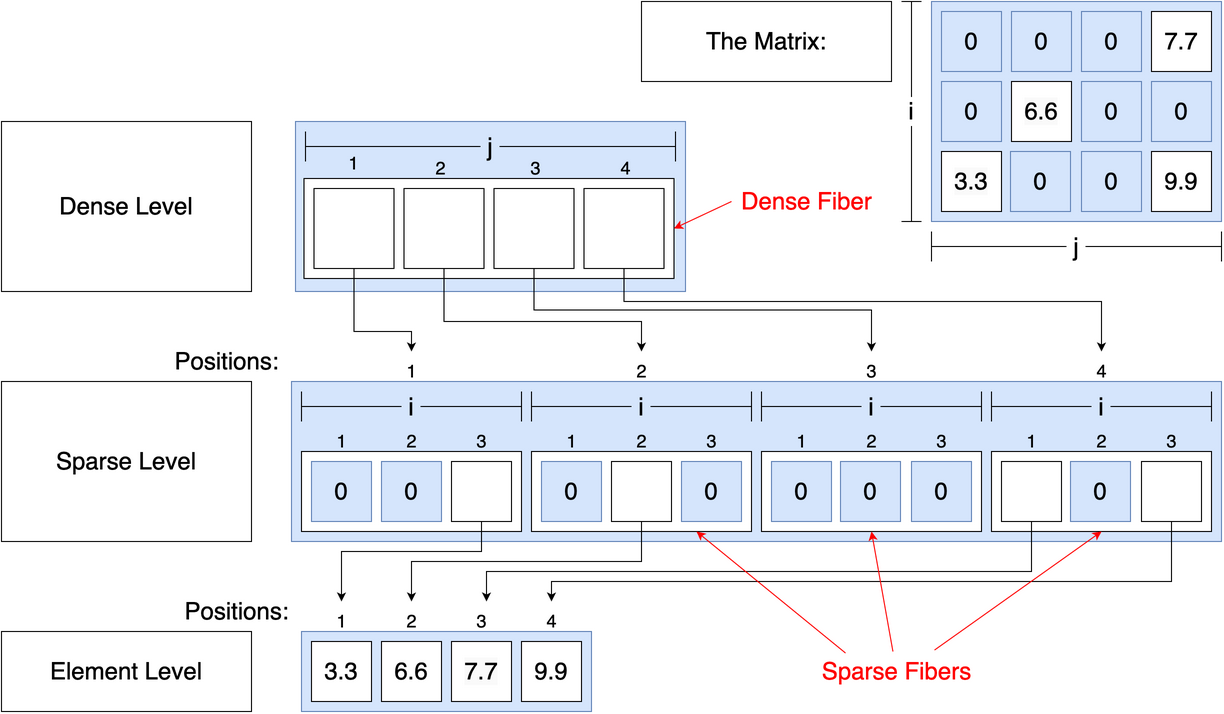
\includegraphics[width=0.45\linewidth]{LevelsVsFibers-matrix.png}\hfill%
    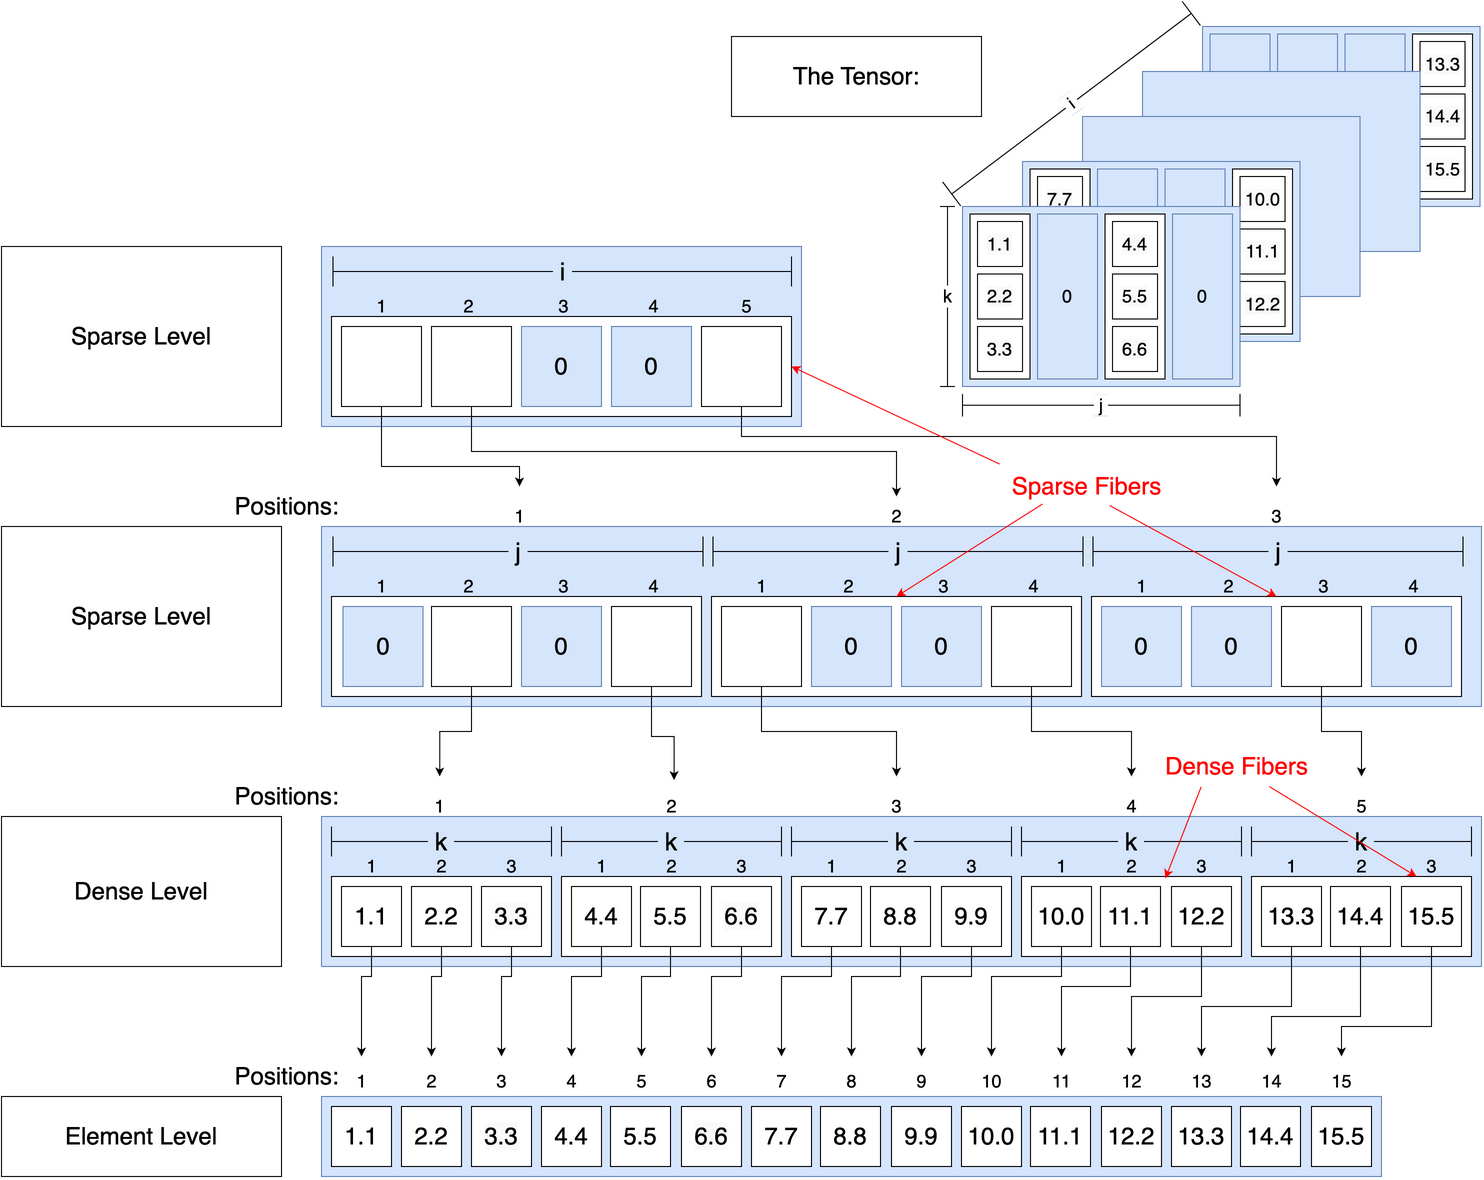
\includegraphics[width=0.5\linewidth]{LevelsVsFibers-tensor.png}
    \caption{Levels and fiber tree representations of a sparse matrix and a sparse tensor. On left, a matrix is represented in a fibertree corresponding to CSC format, with a dense outer level and a sparse inner level. On right, a tensor is represented in a fibertree with two sparse outer levels, and a dense inner level. Note that the element levels in this case form the leaves of the tree.}
    \label{fig:levelsvsfibers}
\end{figure}

\subsection{Tensor Lifecycle, Declare, Freeze, Thaw, Unfurl}

Our simplified view of a level is enabled by our use of looplets to represent
the structure within each fiber. In fact, our level interface requires only
5 highly general operations, described below:

Our view of a level as a fiber allocator implies an allocation function
$assemble(tns, pos_{start}:pos_{stop})$, which allocates fibers at positions
$pos_{start}:pos_{stop}$ in the level. We don't specify a de-allocation function,
instead relying on initialization to reset the fiber if it needs to be reused.

\paragraph{$declare(lvl, init, dims...)$} Declares the level to hold subtensors of size $dims$ and an initial value of $init$. 
\paragraph{$declare(lvl, init, dims...)$} Declares the level to hold subtensors of size $dims$ and an initial value of $init$. 
\paragraph{$freeze(lvl, init, dims...)$} Declares the level to hold subtensors of size $dims$ and an initial value of $init$. 

\subsection{Core Level Language Primitives}
\begin{enumerate}
\item SparseList
\item SparseDict
\item ...
\end{enumerate}


